%  A simple AAU report template.
%  2015-05-08 v. 1.2.0
%  Copyright 2010-2015 by Jesper Kjær Nielsen <jkn@es.aau.dk>
%
%  This is free software: you can redistribute it and/or modify
%  it under the terms of the GNU General Public License as published by
%  the Free Software Foundation, either version 3 of the License, or
%  (at your option) any later version.
%
%  This is distributed in the hope that it will be useful,
%  but WITHOUT ANY WARRANTY; without even the implied warranty of
%  MERCHANTABILITY or FITNESS FOR A PARTICULAR PURPOSE.  See the
%  GNU General Public License for more details.
%
%  You can find the GNU General Public License at <http://www.gnu.org/licenses/>.
%
%  A simple AAU report template.
%  2015-05-08 v. 1.2.0
%  Copyright 2010-2015 by Jesper Kjær Nielsen <jkn@es.aau.dk>
%
%  This is free software: you can redistribute it and/or modify
%  it under the terms of the GNU General Public License as published by
%  the Free Software Foundation, either version 3 of the License, or
%  (at your option) any later version.
%
%  This is distributed in the hope that it will be useful,
%  but WITHOUT ANY WARRANTY; without even the implied warranty of
%  MERCHANTABILITY or FITNESS FOR A PARTICULAR PURPOSE.  See the
%  GNU General Public License for more details.
%
%  You can find the GNU General Public License at <http://www.gnu.org/licenses/>.
%
\documentclass[11pt,letterpaper]{report}
%%%%%%%%%%%%%%%%%%%%%%%%%%%%%%%%%%%%%%%%%%%%%%%%
% Language, Encoding and Fonts
% http://en.wikibooks.org/wiki/LaTeX/Internationalization
%%%%%%%%%%%%%%%%%%%%%%%%%%%%%%%%%%%%%%%%%%%%%%%%
% Select encoding of your inputs. Depends on
% your operating system and its default input
% encoding. Typically, you should use
%   Linux  : utf8 (most modern Linux distributions)
%            latin1
%   Windows: ansinew
%            latin1 (works in most cases)
%   Mac    : applemac
% Notice that you can manually change the input
% encoding of your files by selecting "save as"
% an select the desired input encoding.
\usepackage[utf8]{inputenc}
% Make latex understand and use the typographic
% rules of the language used in the document.
\usepackage[english]{babel}
\usepackage{csquotes}
% Use the palatino font
%\usepackage[sc]{mathpazo}
%\linespread{1.05}         % Palatino needs more leading (space between lines)
% Choose the font encoding
\usepackage[T1]{fontenc}
%%%%%%%%%%%%%%%%%%%%%%%%%%%%%%%%%%%%%%%%%%%%%%%%
% Graphics and Tables
% http://en.wikibooks.org/wiki/LaTeX/Importing_Graphics
% http://en.wikibooks.org/wiki/LaTeX/Tables
% http://en.wikibooks.org/wiki/LaTeX/Colors
%%%%%%%%%%%%%%%%%%%%%%%%%%%%%%%%%%%%%%%%%%%%%%%%
% load a colour package
\usepackage[table, dvipsnames]{xcolor}    % loads also »colortbl«
% \usepackage{xcolor}
% \definecolor{aaublue}{RGB}{33,26,82}% dark blue
% The standard graphics inclusion package
\usepackage{graphicx}
% Set up how figure and table captions are displayed
\usepackage{caption}
\captionsetup{%
  font=footnotesize,% set font size to footnotesize
  labelfont=bf % bold label (e.g., Figure 3.2) font
}
% Make the standard latex tables look so much better
\usepackage{array,booktabs}
% Enable the use of frames around, e.g., theorems
% The framed package is used in the example environment
\usepackage{framed}

%%%%%%%%%%%%%%%%%%%%%%%%%%%%%%%%%%%%%%%%%%%%%%%%
% Mathematics
% http://en.wikibooks.org/wiki/LaTeX/Mathematics
%%%%%%%%%%%%%%%%%%%%%%%%%%%%%%%%%%%%%%%%%%%%%%%%
% Defines new environments such as equation,
% align and split
\usepackage{amsmath}
% Adds new math symbols
\usepackage{amssymb}
% Use theorems in your document
% The ntheorem package is also used for the example environment
% When using thmmarks, amsmath must be an option as well. Otherwise \eqref doesn't work anymore.
\usepackage[framed,amsmath,thmmarks]{ntheorem}

%%%%%%%%%%%%%%%%%%%%%%%%%%%%%%%%%%%%%%%%%%%%%%%%
% Page Layout
% http://en.wikibooks.org/wiki/LaTeX/Page_Layout
%%%%%%%%%%%%%%%%%%%%%%%%%%%%%%%%%%%%%%%%%%%%%%%%
% Change margins, papersize, etc of the document
% \usepackage[
%   inner=28mm,% left margin on an odd page
%   outer=41mm,% right margin on an odd page
%   ]{geometry}
\usepackage[margin=1in]{geometry}
% Modify how \chapter, \section, etc. look
% The titlesec package is very configureable
\usepackage{titlesec}
\titleformat{\chapter}[display]{\normalfont\huge\bfseries}{\chaptertitlename\ \thechapter}{20pt}{\Huge}
\titleformat*{\section}{\normalfont\Large\bfseries}
\titleformat*{\subsection}{\normalfont\large\bfseries}
\titleformat*{\subsubsection}{\normalfont\normalsize\bfseries}
%\titleformat*{\paragraph}{\normalfont\normalsize\bfseries}
%\titleformat*{\subparagraph}{\normalfont\normalsize\bfseries}

% Clear empty pages between chapters
\let\origdoublepage\cleardoublepage
\newcommand{\clearemptydoublepage}{%
  \clearpage
  {\pagestyle{empty}\origdoublepage}%
}
\let\cleardoublepage\clearemptydoublepage

% Change the headers and footers
\usepackage{fancyhdr}
\pagestyle{fancy}
\fancyhf{} %delete everything
\renewcommand{\headrulewidth}{0pt} %remove the horizontal line in the header
%\fancyhead[RE]{\small\nouppercase\leftmark} %even page - chapter title
\fancyhead[L]{\small\nouppercase\rightmark} %uneven page - section title
\fancyhead[R]{\thepage} %page number on all pages
% Do not stretch the content of a page. Instead,
% insert white space at the bottom of the page
\raggedbottom
% Enable arithmetics with length. Useful when
% typesetting the layout.
\usepackage{calc}

%%%%%%%%%%%%%%%%%%%%%%%%%%%%%%%%%%%%%%%%%%%%%%%%
% Bibliography
% http://en.wikibooks.org/wiki/LaTeX/Bibliography_Management
%%%%%%%%%%%%%%%%%%%%%%%%%%%%%%%%%%%%%%%%%%%%%%%%
\usepackage[backend=bibtex,
  bibencoding=utf8
  ]{biblatex}
\addbibresource{bib/mybib}

%%%%%%%%%%%%%%%%%%%%%%%%%%%%%%%%%%%%%%%%%%%%%%%%
% Misc
%%%%%%%%%%%%%%%%%%%%%%%%%%%%%%%%%%%%%%%%%%%%%%%%
% Add bibliography and index to the table of
% contents
\usepackage[nottoc]{tocbibind}
% Add the command \pageref{LastPage} which refers to the
% page number of the last page
\usepackage{lastpage}
% Add todo notes in the margin of the document
\usepackage[
%  disable, %turn off todonotes
  colorinlistoftodos, %enable a coloured square in the list of todos
  textwidth=\marginparwidth, %set the width of the todonotes
  textsize=scriptsize, %size of the text in the todonotes
  color=orange!70,
  ]{todonotes}

%%%%%%%%%%%%%%%%%%%%%%%%%%%%%%%%%%%%%%%%%%%%%%%%
% Hyperlinks
% http://en.wikibooks.org/wiki/LaTeX/Hyperlinks
%%%%%%%%%%%%%%%%%%%%%%%%%%%%%%%%%%%%%%%%%%%%%%%%
% Enable hyperlinks and insert info into the pdf
% file. Hypperref should be loaded as one of the
% last packages
\usepackage{hyperref}
\hypersetup{%
	pdfpagelabels=true,%
	hidelinks,
	plainpages=false,%
	pdfauthor={Author(s)},%
	pdftitle={Title},%
	pdfsubject={Subject},%
	bookmarksnumbered=true,%
	colorlinks=false,%
	citecolor=black,%
	filecolor=black,%
	linkcolor=black,% you should probably change this to black before printing
	urlcolor=black,%
	pdfstartview=FitH%
}

\usepackage{enumitem}

\usepackage{booktabs}% http://ctan.org/pkg/booktabs
\newcommand{\tabitem}{~~\llap{\textbullet}~~}

% \usepackage[textwidth = 155mm]{geometry}
\usepackage{tabularx}

\usepackage{listings}
\usepackage{times}
\usepackage{textcomp}

\newcommand{\studentComment}[1]{\todo[inline,color=ForestGreen!70]{#1}}
\newcommand{\foxComment}[1]{\todo[inline]{#1}}

\usepackage{setspace}

% \usepackage[demo]{graphicx} % "demo" option just for this example
\usepackage{subcaption}
% package inclusion and set up of the document
% see, e.g., http://en.wikibooks.org/wiki/LaTeX/Formatting#Hyphenation
% for more information on word hyphenation
\hyphenation{ex-am-ple hy-phen-a-tion short}
\hyphenation{long la-tex}%
%  A simple AAU report template.
%  2015-05-08 v. 1.2.0
%  Copyright 2010-2015 by Jesper Kjær Nielsen <jkn@es.aau.dk>
%
%  This is free software: you can redistribute it and/or modify
%  it under the terms of the GNU General Public License as published by
%  the Free Software Foundation, either version 3 of the License, or
%  (at your option) any later version.
%
%  This is distributed in the hope that it will be useful,
%  but WITHOUT ANY WARRANTY; without even the implied warranty of
%  MERCHANTABILITY or FITNESS FOR A PARTICULAR PURPOSE.  See the
%  GNU General Public License for more details.
%
%  You can find the GNU General Public License at <http://www.gnu.org/licenses/>.
%
%
%
% see, e.g., http://en.wikibooks.org/wiki/LaTeX/Customizing_LaTeX#New_commands
% for more information on how to create macros

%%%%%%%%%%%%%%%%%%%%%%%%%%%%%%%%%%%%%%%%%%%%%%%%
% Macros for the titlepage
%%%%%%%%%%%%%%%%%%%%%%%%%%%%%%%%%%%%%%%%%%%%%%%%
%Creates the aau titlepage
\newcommand{\aautitlepage}[3]{%
  {
    %set up various length
    \ifx\titlepageleftcolumnwidth\undefined
      \newlength{\titlepageleftcolumnwidth}
      \newlength{\titlepagerightcolumnwidth}
    \fi
    \setlength{\titlepageleftcolumnwidth}{0.5\textwidth-\tabcolsep}
    \setlength{\titlepagerightcolumnwidth}{\textwidth-2\tabcolsep-\titlepageleftcolumnwidth}
    %create title page
    \thispagestyle{empty}
    \noindent%
    \begin{tabular}{@{}ll@{}}
      \parbox{\titlepageleftcolumnwidth}{
        \iflanguage{danish}{%
          
\includegraphics[width=\titlepageleftcolumnwidth]{figures/aau_logo_da}
        }{%
          
\includegraphics[width=\titlepageleftcolumnwidth]{figures/vt-logo}
        }
      } &
      \parbox{\titlepagerightcolumnwidth}{\raggedleft\sf\small
        #2
      }\bigskip\\
       #1 &
      \parbox[t]{\titlepagerightcolumnwidth}{%
      \textbf{Abstract:}\bigskip\par
        \fbox{\parbox{\titlepagerightcolumnwidth-2\fboxsep-2\fboxrule}{%
          #3
        }}
      }\\
    \end{tabular}
    \vfill
    \iflanguage{danish}{%
      \noindent{\footnotesize\emph{Rapportens indhold er frit tilgængeligt, men offentliggørelse (med kildeangivelse) må kun ske efter aftale med forfatterne.}}
    }{%
      \noindent{\footnotesize\emph{The content of this report is freely available, but publication (with reference) may only be pursued due to agreement with the author.}}
    }
    \clearpage
  }
}

%Create english project info
\newcommand{\englishprojectinfo}[8]{%
  \parbox[t]{\titlepageleftcolumnwidth}{
    \textbf{Title:}\\ #1\bigskip\par
    \textbf{Theme:}\\ #2\bigskip\par
    \textbf{Project Period:}\\ #3\bigskip\par
    \textbf{Project Group:}\\ #4\bigskip\par
    \textbf{Participant(s):}\\ #5\bigskip\par
    \textbf{Supervisor(s):}\\ #6\bigskip\par
    \textbf{Copies:} #7\bigskip\par
    \textbf{Page Numbers:} \pageref{LastPage}\bigskip\par
    \textbf{Date of Completion:}\\ #8
  }
}

%Create danish project info
\newcommand{\danishprojectinfo}[8]{%
  \parbox[t]{\titlepageleftcolumnwidth}{
    \textbf{Titel:}\\ #1\bigskip\par
    \textbf{Tema:}\\ #2\bigskip\par
    \textbf{Projektperiode:}\\ #3\bigskip\par
    \textbf{Projektgruppe:}\\ #4\bigskip\par
    \textbf{Deltager(e):}\\ #5\bigskip\par
    \textbf{Vejleder(e):}\\ #6\bigskip\par
    \textbf{Oplagstal:} #7\bigskip\par
    \textbf{Sidetal:} \pageref{LastPage}\bigskip\par
    \textbf{Afleveringsdato:}\\ #8
  }
}

%%%%%%%%%%%%%%%%%%%%%%%%%%%%%%%%%%%%%%%%%%%%%%%%
% An example environment
%%%%%%%%%%%%%%%%%%%%%%%%%%%%%%%%%%%%%%%%%%%%%%%%
\theoremheaderfont{\normalfont\bfseries}
\theorembodyfont{\normalfont}
\theoremstyle{break}
\def\theoremframecommand{{\color{gray!50}\vrule width 5pt \hspace{5pt}}}
\newshadedtheorem{exa}{Example}[chapter]
\newenvironment{example}[1]{%
		\begin{exa}[#1]
}{%
		\end{exa}
}% my new macros

\pagestyle{empty}

\setlength{\parskip}{2ex plus 0.5ex minus 0.2ex}
\setlength{\parindent}{0pt}

\makeatletter  %to avoid error messages generated by "\@". Makes Latex treat "@" like a letter

\linespread{1.5}
\def\submitdate#1{\gdef\@submitdate{#1}}

\def\maketitle{
  \begin{titlepage}{
    %\linespread{1.5}
    \Large University of London \\
    %\linebreak
    Imperial College of Science, Technology and Medicine \\
    %\linebreak
    Department of Computing
    \rm
    \vskip 3in
    \Large \bf \@title \par
  }
  \vskip 0.3in
  \par
  {\Large \@author}
  \vskip 4in
  \par
  Submitted in part fulfilment of the requirements for the degree of
  \linebreak
  Doctor of Philosophy in Computing of the University of London and
  \linebreak
  the Diploma of Imperial College, \@submitdate
  \vfil
  \end{titlepage}
}

\def\titlepage{
  \newpage
  \centering
  \linespread{1}
  \normalsize
  \vbox to \vsize\bgroup\vbox to 9in\bgroup
}
\def\endtitlepage{
  \par
  \kern 0pt
  \egroup
  \vss
  \egroup
  \cleardoublepage
}

\def\abstract{
  \begin{center}{
    \large\bf Abstract}
  \end{center}
  \small
  %\def\baselinestretch{1.5}
  \linespread{1.5}
  \normalsize
}
\def\endabstract{
  \par
}

\newenvironment{acknowledgements}{
  \cleardoublepage
  \begin{center}{
    \large \bf Acknowledgements}
  \end{center}
  \small
  \linespread{1.5}
  \normalsize
}{\cleardoublepage}
\def\endacknowledgements{
  \par
}

\newenvironment{dedication}{
  \cleardoublepage
  \begin{center}{
    \large \bf Dedication}
  \end{center}
  \small
  \linespread{1.5}
  \normalsize
}{\cleardoublepage}
\def\enddedication{
  \par
}

\def\preface{
    \pagenumbering{roman}
    \pagestyle{plain}
    \doublespacing
}

\def\body{
    \cleardoublepage
    \pagestyle{uheadings}
    \tableofcontents
    \pagestyle{plain}
    \cleardoublepage
    \pagestyle{uheadings}
    \listoftables
    \pagestyle{plain}
    \cleardoublepage
    \pagestyle{uheadings}
    \listoffigures
    \pagestyle{plain}
    \cleardoublepage
    \pagestyle{uheadings}
    \pagenumbering{arabic}
    \doublespacing
}

\makeatother  %to avoid error messages generated by "\@". Makes Latex treat "@" like a letter

\begin{document}
  %frontmatter
  \pagestyle{empty} %disable headers and footers
  \pagenumbering{roman} %use roman page numbering in the frontmatter
  %  A simple AAU report template.
%  2015-05-08 v. 1.2.0
%  Copyright 2010-2015 by Jesper Kjær Nielsen <jkn@es.aau.dk>
%
%  This is free software: you can redistribute it and/or modify
%  it under the terms of the GNU General Public License as published by
%  the Free Software Foundation, either version 3 of the License, or
%  (at your option) any later version.
%
%  This is distributed in the hope that it will be useful,
%  but WITHOUT ANY WARRANTY; without even the implied warranty of
%  MERCHANTABILITY or FITNESS FOR A PARTICULAR PURPOSE.  See the
%  GNU General Public License for more details.
%
%  You can find the GNU General Public License at <http://www.gnu.org/licenses/>.
%
\pdfbookmark[0]{Front page}{label:frontpage}%
\begin{titlepage}
  \addtolength{\hoffset}{0.5\evensidemargin-0.5\oddsidemargin} %set equal margins on the frontpage - remove this line if you want default margins
  \noindent%
  \begin{center}
    
\includegraphics[width=0.5\textwidth-\tabcolsep]{figures/vt-logo} \\
  \end{center}
  \vspace{0.5cm}
  \begin{center}
    {\Large
      CS 5604 Information Storage and Retrieval \\
      Spring 2016\\
    }
    \vspace{0.2cm}
    {\large
      Interim Report 3%Insert document type (e.g., Project Report)
    }
  \end{center}
  \vspace{0.2cm}
  \begin{tabular}{@{}p{\textwidth}@{}}
    \toprule[2pt]
    \midrule
    \vspace{0.2cm}
    \begin{center}
    \Huge{\textbf{
      Text Classification% insert your title here
    }}
    \end{center}
    \vspace{0.2cm}\\
    \midrule
    \toprule[2pt]
  \end{tabular}
  \vspace{2 cm}
  \begin{center}
    {\Large
      Team Members:\\
    }
    \vspace{0.2cm}
    {\large
      Hossameldin Shahin <hshahin@vt.edu>\\
      Matthew Bock <mattb93@vt.edu>\\
      Michael Cantrell <mcantrell@vt.edu>\\
    }
  \end{center}
  \vfill
  \begin{center}
    {\Large
      Project Advisor:\\
    }
    \vspace{0.2cm}
    {\large
      Prof. Edward A. Fox\\
    }
  \end{center}
  \vfill
  \begin{center}
    {\Large
      3/31/2016\\
      Virginia Tech, Blacksburg\\
    }
  \end{center}
\end{titlepage}
\clearpage
  \addcontentsline{toc}{chapter}{Abstract}

\begin{abstract}
In the grand scheme of a large Information Retrieval project, the work of our team will be that of performing text classification on both the tweet collections and their associated webpages. In order to accomplish this task, we will seek to complete three primary goals. We will begin by performing research to determine the best way to extract information that will be used to represent a given document. Following that, we will work to determine the best method to select features and then construct feature vectors. Our final goal is to use the information gathered previously to build an effective way to classify each document in the tweet and webpage collections. We intend for these classifiers to be built with consideration of the ontology developed for the IDEAL project.

The team assigned to perform this classification work last year researched various methods and tools that could be useful in accomplishing the goals we have set forth. Last year's team developed a system that was able to accomplish similar goals to those we have set forth with a promising degree of success. Our goal for this year is to improve upon their successes using new technologies such as Apache Spark. It is our hope that this will allow us to build a more optimized system capable of working with larger collections of tweets and webpages.

We also have several other goals for this semester's work in addition to improving on prior classification work. Two of those main goals include handling incremental data updates and performing evaluations as to the effectiveness of our classification system. We have designed our system with both of these in mind. Our approach to both of these goals are described in detail in this paper.

\foxComment{Should add about: incremental, running experiments, evaluations.}

\end{abstract}
  \cleardoublepage

\addcontentsline{toc}{chapter}{Acknowledgements}

\begin{acknowledgements}

I would like to express (whatever feelings I have) to:

\begin{itemize}
 \item My supervisor
 \vspace*{3mm}
 \item My second supervisor
 \vspace*{3mm}
 \item Other researchers
 \vspace*{3mm}
 \item My family and friends
\end{itemize}

\end{acknowledgements}

  \cleardoublepage

  \pdfbookmark[0]{Contents}{label:contents}
  \pagestyle{fancy} %enable headers and footers again
  \tableofcontents
  \listoffigures
  \listoftables

  \cleardoublepage

  %mainmatter
  \pagenumbering{arabic} %use arabic page numbering in the mainmatter
  \chapter{Introduction}\label{ch:introduction}
%\studentComment{Miscommunication with Solr. Also assumed we were doing redundant work on the clean up part.}

The classification team’s goal is to take collections of tweets and webpages and classify them based on their relevance to given classes or topics. Our team fits into the grand scheme of the project by working between the Collection Management team and the Solr team. The Collection Management team will be responsible for taking the raw tweet and webpage data and filtering out any obvious spam, vulgarity, or otherwise unreadable and unwanted content. The Collection Management team will write the cleaned data into a table in our HBase instance. Once this is done, we will attempt to classify each document's relevance to a specific category. We will explore several methods for accomplishing this, starting with the methodology laid out by last year's Classification team \cite{cui2015classification}. Once we have classified the data, we will be able to pass it along to the Solr team by writing the newly classified data back into the primary HBase table as a column family. The Solr team will then be able to use the column family in the indexing of all the tweet and webpage data. Solr will then provide the indexes for the data to the Front End team, allowing anyone to make use to the system we are creating.
%The Solr team will import our classified data into the Solr system, making it accessible to anyone using the system we are creating.

This paper represents the fourth interim report from the Classification team working as a part of the larger scale project for CS5604 Information Storage and Retrieval. The current state of the work is a partial draft of the final report; therefore expect further additions and details in some chapters as the course progresses.

We begin by documenting our understanding of some of the pertinent literature, namely the course textbook and the Classification team report from last year; this can be found in Chapter \ref{ch:literatureReview}, our literature review. Chapter \ref{ch:ReqDesignImp} is the primary section of the document and includes our discussion of the project requirements, an outline for our design for the classification portion of the larger project, and finally a breakdown of our current progress and future plans for the text classification project.

These chapters are then followed by a User Manual in Chapter \ref{ch:userManual}, where we will discuss details in which a user of our methods and programs would have interest. We then include a separate Developer Manual in Chapter \ref{ch:developerManual}, which will document and include details of the code base so that it might be extended and leveraged by other developers.

Following this we include our conclusions about the state of the project thus far and present our thoughts for future work in Chapter \ref{ch:futureWork}.

  \chapter{Literature Review}\label{ch:literatureReview}

\section{Textbook}
The textbook \cite{manning2008introduction} introduces the classification problem. That is, given a set of classes, the goal is to determine what subset of those classes a document may belong to. To that end, the textbook describes a number of methodologies for selecting features. These features are then used by one of the classification methods discussed. The primary methods discussed are Na\"{i}ve Bayes, Vector Space Classification, and the Support Vector Machine.

\section{Papers}
The primary paper that has been used as a reference is the final report of the Classification team from last year \cite{cui2015classification}. We have read through this report to understand the progress that the Classification team made last year as well as using the paper to gain an understanding of the task and interactions of the systems that we are using to perform our work. At a high level, the paper described a methodology employed by the team in which they were able to apply the Na{\"i}ve Bayes method to classify sets of data. The team used Apache Mahout machine learning technology to generate Na{\"i}ve Bayes classifiers to make predictions for new data. The biggest difference from last year's work to this year's work is that we will be primarily using Apache Spark, and so while we will be able to reference their work, we are using entirely different technologies and will need to modify our approach accordingly.

Initially, we attempted an approach where we would issue queries to Solr to build a set of training data for a classifier. However, we were informed by the GRAs that this approach would not work because the Solr API was not exposed on the cluster, and so we would not be able to access it. When we started looking into new approaches, we were advised to look at Frequent Pattern Mining (FPM). We have looked at a paper by Han et al.\ \cite{han2000mining}, which presents a novel frequent pattern tree (FP-tree) structure and FP-tree based mining method called FP-growth. This method allows for mining the complete set of frequent patterns by pattern fragment growth. In this paper they also demonstrate that their new method is an order of magnitude faster than the typical apriori algorithm. The paper goes on to compare the performance against other popular data mining algorithms and discusses the use of the algorithm on some large industrial databases. We are currently making use of the FP-growth algorithm and data structure in our working classification prototype.
  \chapter[Requirements, Design, and Implementation]{Requirements, Design, And\\ Implementation}\label{ch:ReqDesignImp}
\section{Requirements}
Based upon group discussions in a classroom setting, it was decided what information that the Collection Management team would provide to the other teams that need to work with cleaned tweet data. A full specification of these decisions can be found by viewing the Collection Management team's report; however we will briefly discuss the points that were relevant to us.

Given the cleaned tweet data from Collection Management, our team will then be able to perform the methodologies we describe later to classify whether a document is relevant or non-relevant to a given class. A detailed layout of the project with our interactions highlighted is provided by Figure \ref{fig:design}.

We will then place our classification information in the HBase datastore to mark the relevance of each document. The Solr team will then index this class information that we provide, allowing for more robust query results and more useful facets to be created.

\begin{figure}[ht]
	\centering
	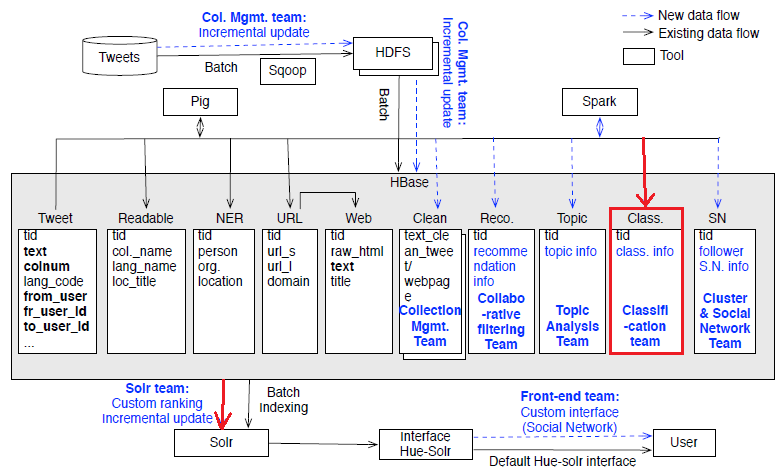
\includegraphics[width=\textwidth]{figures/data_flow.png}
    \caption{Layout of the project teams, as provided by Professor Fox and his GRAs.}\label{fig:design}
\end{figure}

\section{Design}
Our current design is based primarily off of recommendations from the GRAs assisting the class. We have also taken substantial input from last year's Classification team \cite{cui2015classification} and the Professor.

We have designed our current solution around pulling training data from and testing on a small collection of around 100,000 tweets. This was originally going to be performed on the small collection that was assigned to our team, \texttt{\#germanwings}. However, due to some changes and discussion among the other teams, we have decided to continue with designing and testing our solution using a cleaned dataset provided by the Collection Management team. However this dataset was not made available until after our current solution was mostly implemented using our original small dataset. Therefore for the rest of this document we will be using the small dataset \texttt{z\_602}, \texttt{\#germanwings}. All future work will be done using cleaned data from the Collection Management team.

\section{Implementation}
Our implementation can be easily laid out in a step by step workflow, with only one step requiring true manual input and evaluation from a person. Figure \ref{fig:overview} illustrates the general flow of data that we have implemented thus far. Below we will discuss each step in detail.

Our methodology primarily revolves around building a training set. This training set will be used for training a machine learning model, a.k.a. a classifier.

\begin{figure}[ht]
	\centering
	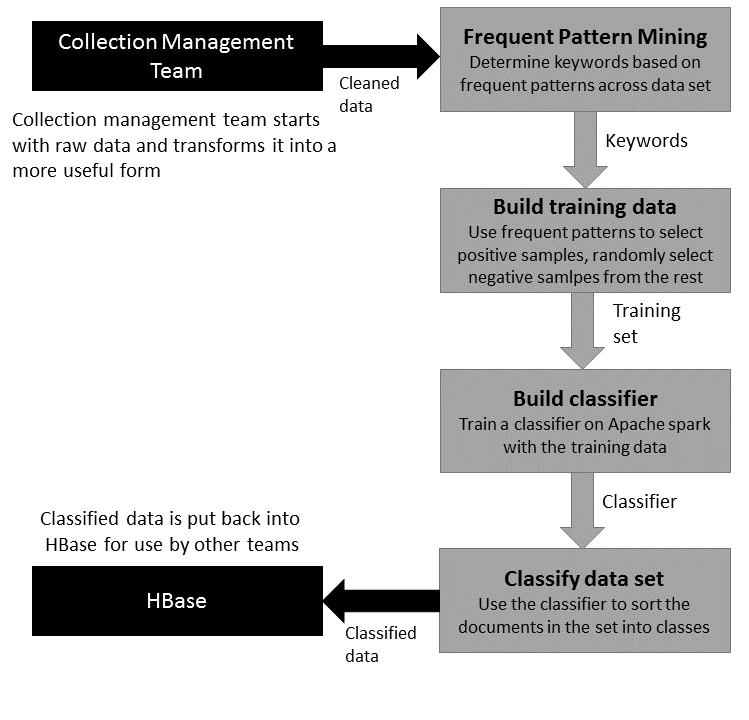
\includegraphics[scale=.65]{figures/design_flow_chart.png}
    \caption{High level overview of the flow of data through the classification system.}\label{fig:overview}
\end{figure}

\subsection{Environment Set--Up}
Our group decided to avoid working directly on the cluster, granting us full administrative rights to a machine, which allowed us to set up and test different configurations and algorithms beyond what might currently be supported by the Hadoop cluster being used for class.

A prime example, and the primary motivating factor for our choice, was our decision to use Frequent Pattern Mining (FPM) in the construction of our training sets. The cluster provided for the class was running Spark version 1.2.0, but FPM is not supported by Spark until version 1.5.0. Since FPM was a methodology suggested by the GRAs, and they assured us that they could upgrade the cluster to a more current version of Spark, we decided to proceed with this method.

Due to time constraints, we created a Debian Virtual Machine with sufficient specs to begin writing and testing our methodology. This machine is hosted on a VMware vSphere cluster that belongs to the Virginia Tech IT Security Office/Lab. Since one of the group members works in this lab, we were able to provision this VM. It has been assigned 32 GB of RAM, 16 processor cores, and 40 GB of storage. This has proven to be more than adequate for the testing that we have performed on our small data set.

The Hadoop cluster has now been upgraded to Spark 1.5.0 allowing us to transition our code and methods over and work directly with the HBase instance. As this was a recent change, we are still in the process of this transition and cannot report on what effect it will have, i\. e\. whether there are any issues encountered that break our implementation.

\subsection{Building the Training Data}
In order to begin the classification process we have to prepare a set of training data to use for the machine learning classification algorithm. In order to do this, we assume that we are working with data that has been cleaned of profanity and non-printable characters.

For our methodology we then need to take the content of each tweet and webpage as a string and tokenize it. This means that we will remove any duplicate words and have the result be a set of the vocabulary in the tweet (or webpage). At this stage we also remove any stop words that are in the vocabulary to make sure our algorithms in the next phase are not skewed by taking stop words into account. During this phase we also strip the \# from any hashtags that are present in the tweet.

In our initial design and testing we did not yet have access to cleaned tweets and webpages from the Collection Management team, so we worked primarily to build the methodology that would be used once those resources became available. Therefore, some of the steps mentioned previously, such as the removal of the stop words and the removal of the \# from hashtags are unnecessary when working with the data provided by Collection Management in HBase.

The next step in our algorithm involves the use of Frequent Pattern Mining (FPM) to determine the most frequently used patterns of words in the text of a series of tweets or webpages. FPM looks at the set of existing vocabulary for each text and determines which tokens appear together within a tweet's vocabulary most often.

This is the stage where manual intervention in necessary. We look at a file containing a sorted list of all the frequent pattern;, from this we choose a set of features to train on. In our attempts at training a classifier for our small data collection, we chose to select a frequent pattern of four words. This was essentially an arbitrary choice, but we believe that it strikes a good balance between being too specific and missing some relevant tweets and being too broad and pulling in a number of irrelevant tweets.

At this stage we need to create positive and negative training samples. To do this, we pull a random subset of tweets that contain our frequent pattern and classify those as positive samples. For our negative sample we pull a random subset of tweets that do not contain our frequent pattern. To ensure that this labeling is at least mostly correct, we will inspect both the positive and negative training sets (or a portion of them) to confirm that each set is composed of either relevant tweets and webpages or non-relevant ones as appropriate. If in this inspection we find that the choice of frequent pattern has generated a poor training set, we will choose a different frequent pattern and go through the process again.

%\todo[inline]{Have you checked whether the results of using FPM to determine labeling of tweets as positive or negative is correct?  That is, did you manually check (some) of the label assignments?  Will you use the same approach for webpages too?}For our negative sample we pull a random subset of tweets that do not contain our frequent pattern.

\subsection{Training the Classifier}

We then use the sets of positive and negative samples to train a classifier. We are currently using a logistic regression classifier in our implementation, primarily due to its ease of implementation in Spark.

FPM allows us to develop a training set by filtering the tweets and webpages down to some subset of those that do and do not contain the selected frequent patterns. We take these subsets as the positive training data and the negative training data.

At this point we then feed the selected documents into the classifier; this step uses all the words in each document of the training data, not just the words used for FPM. As we progress we intend to try using several different classifiers to determine which one provides us with the best results.

%As the project progresses we \todo[inline]{When you try other classifiers, will you use the same training data?  When you use LR and those others, what are the features - just those from FPM, or all words in the labeled documents?}plan to attempt using several different classifiers and comparing their effectiveness at classifying our data.

\subsection{Predicting the Class}

After training the classifier, we apply the classifier to all the tweets across our small data collection. This results in a binary scoring for each tweet as relevant or non-relevant to the collection based upon the training data we selected.

\subsection{Evaluating the Classifier}

We can evaluate the accuracy of our model by judging how well it classifies some of the data that could have been in our positive or negative samples. This is the most intuitive evaluation however it requires a great deal of manual effort to perform. We need to pull out a sampling of classified data and look through it manually; marking whether or not the classification was correct.

Another evaluation that we can perform looks at how well each small collection does at being relevant to the topic at hand. If a large number of the documents in the collection are classified as non-relevant, than the collection as a whole has not done a good job capturing the event in question.

Finally, we need to perform an evaluation of how well our method of using FPM to determine the training documents works. This is much like the first evaluation in that it can be very manual. We will need to dump the generated training sets out to files and then manually decide whether a given set has all (or primarily) relevant or non-relevant documents, as appropriate.


%\todo[inline]{When you mention about not well implemented, does that mean: you are not sure how to do this, you have not done it, you did it but had problems, etc.? Where is the evaluation plan detailed?}We currently do not have this well implemented, but plan to have this evaluation completed before the next report.

\subsection{Interfacing with HBase}

We are currently able to process the six small data files and determine whether or not each tweet in the collection is relevant or irrelevant. However, at the time of this writing, our python scripts are unable to write data directly back to HBase (but that will change soon now that the cluster's software has been updated). To work around this, we have made use of HBase's ImportTSV functionality to manually put our processed data into the table.

\begin{figure}[ht]
	\centering
	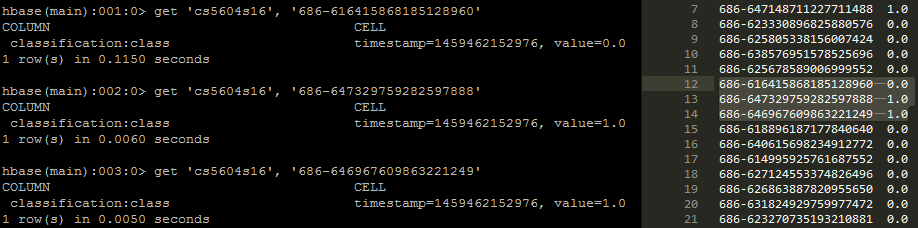
\includegraphics[scale=.65]{figures/hbase-data.png}
    \caption{An example .tsv file (right) that has been imported into HBase. The values of the highlighted entries are shown as outputs of HBase's "get" command on the left.}\label{fig:hbase-data}
\end{figure}

As shown in Figure \ref{fig:hbase-data}, for each of the data sets we have produced a .tsv file with two columns: one containing the tweet id (which serves as the row key in HBase), and one containing either 1.0 or 0.0 depending on whether the tweet was relevant or irrelevant (respectively) to the category. These six files have been imported into HBase and are ready for use by the other project teams. Within HBase, we have created a column family named "classification." Within our column family, we only have need of one column, named "class." This column is where the 1.0 or 0.0 for each document in the database will be stored for access by other teams.

In the future, we plan to further automate the data processing system by having our python scripts read cleaned data provided by the collection management team straight from the HBase table, and writing our results right back to the table as they are processed. This will enable more efficient classification of any future data that gets indexed into the system.




% Here is the introduction. The next chapter is chapter~\ref{ch:ch2label}.


% a new paragraph


% \section{Examples}
% You can also have examples in your document such as in example~\ref{ex:simple_example}.
% \begin{example}{An Example of an Example}
%   \label{ex:simple_example}
%   Here is an example with some math
%   \begin{equation}
%     0 = \exp(i\pi)+1\ .
%   \end{equation}
%   You can adjust the colour and the line width in the {\tt macros.tex} file.
% \end{example}

% \section{How Does Sections, Subsections, and Subsections Look?}
% Well, like this
% \subsection{This is a Subsection}
% and this
% \subsubsection{This is a Subsubsection}
% and this.

% \paragraph{A Paragraph}
% You can also use paragraph titles which look like this.

% \subparagraph{A Subparagraph} Moreover, you can also use subparagraph titles which look like this\todo{Is it possible to add a subsubparagraph?}. They have a small indentation as opposed to the paragraph titles.

% \todo[inline,color=green]{I think that a summary of this exciting chapter should be added.}
  \chapter{User Manual}\label{ch:userManual}

\section{Installing Requirements}

\section{Preparing the Server}

\section{Using the IPython Notebook}

\subsection{Using the Configuration File}

\subsection{Selecting a Frequent Pattern}

\subsection{Building a Training Set}

\subsection{Training a Classifier}

\subsection{Running the Classifier}

% Here is the introduction. The next chapter is chapter~\ref{ch:ch2label}.


% a new paragraph


% \section{Examples}
% You can also have examples in your document such as in example~\ref{ex:simple_example}.
% \begin{example}{An Example of an Example}
%   \label{ex:simple_example}
%   Here is an example with some math
%   \begin{equation}
%     0 = \exp(i\pi)+1\ .
%   \end{equation}
%   You can adjust the colour and the line width in the {\tt macros.tex} file.
% \end{example}

% \section{How Does Sections, Subsections, and Subsections Look?}
% Well, like this
% \subsection{This is a Subsection}
% and this
% \subsubsection{This is a Subsubsection}
% and this.

% \paragraph{A Paragraph}
% You can also use paragraph titles which look like this.

% \subparagraph{A Subparagraph} Moreover, you can also use subparagraph titles which look like this\todo{Is it possible to add a subsubparagraph?}. They have a small indentation as opposed to the paragraph titles.

% \todo[inline,color=green]{I think that a summary of this exciting chapter should be added.}
  \chapter{Developer Manual}\label{ch:developerManual}

\section{Techniques}

\subsection{Frequent Pattern Mining}

\subsection{Na{\"i}ve Bayes}

\section{}

% Here is the introduction. The next chapter is chapter~\ref{ch:ch2label}.


% a new paragraph


% \section{Examples}
% You can also have examples in your document such as in example~\ref{ex:simple_example}.
% \begin{example}{An Example of an Example}
%   \label{ex:simple_example}
%   Here is an example with some math
%   \begin{equation}
%     0 = \exp(i\pi)+1\ .
%   \end{equation}
%   You can adjust the colour and the line width in the {\tt macros.tex} file.
% \end{example}

% \section{How Does Sections, Subsections, and Subsections Look?}
% Well, like this
% \subsection{This is a Subsection}
% and this
% \subsubsection{This is a Subsubsection}
% and this.

% \paragraph{A Paragraph}
% You can also use paragraph titles which look like this.

% \subparagraph{A Subparagraph} Moreover, you can also use subparagraph titles which look like this\todo{Is it possible to add a subsubparagraph?}. They have a small indentation as opposed to the paragraph titles.

% \todo[inline,color=green]{I think that a summary of this exciting chapter should be added.}
  \chapter{Plan}\label{ch:plan}
%\studentComment{Fix a lack of description on the management of the team work}
%\studentComment{Provide breakdown of individuals contributions}

Our work on this project will happen in two phases. In the first phase, we will attempt to create an initial prototype working with a small set of sample data. This phase will be accomplished mainly in our own external environment so that we can experiment more freely with the technologies to gain a better understanding of how they work and interact together. 

Phase two of the project will involve taking the work done in phase one and expanding it out to the other small sets of data provided to us, and eventually to larger data sets. We will explore other potential techniques as we deem them necessary. This phase will also include a definition and implementation of an evaluation approach. Phase one is small enough that we feel a subjective evaluation is sufficient, but as we expand it will become essential to have a more concrete, quantitative measure of effectiveness.

Please see Table \ref{table:plan} for a weekly breakdown of work.

\rowcolors{2}{gray!25}{white}
\begin{table}
\caption{Weekly breakdown of work to be done.}\label{table:plan}
\begin{tabularx}{155mm}{|>{\setlength\hsize{.2\hsize}\setlength\linewidth{\hsize}}X|>{\setlength\hsize{.3\hsize}\setlength\linewidth{\hsize}}X|>{\setlength\hsize{1.5\hsize}\setlength\linewidth{\hsize}}X|}
	\rowcolor{gray!50}
%\multicolumn{3}{|c|}{Classification of the criticel point $(0,0)$ of $x'=Ax,|\mathbf{A}|\not=0$.}\\
\hline
\centering Weeks & \centering End Date & Tasks \\
\hline

Week 1
&
22 Jan.
&
Understanding the classification task\\
\hline

Week 2
&
29 Jan.
&
\begin{itemize}
\item Understanding the classification task
\item Read about \href{https://canvas.vt.edu/courses/21271/files/folder/2015/Tutorials?preview=390175}{Hadoop streaming using Python}
\end{itemize}\\
\hline

Week 3
&
5 Feb.
&
Start online tutorials about Hadoop and Apache Spark.\cite{pythonSparkTutorial}\cite{solrTeamTutorial}\\
\hline

Week 4
&
12 Feb.
&
Continue online tutorials about Hadoop and Apache Spark.\cite{hbaseShellTutorial}\\
\hline

Week 5
&
19 Feb.
&
\textbf{Phase 1 will include only tweets small data set:}
\begin{itemize}
\item Understanding the classification task
\item Read about Hadoop streaming using python
\end{itemize}\\
\hline

Week 6
&
26 Feb.
&
\begin{itemize}
\item Prepare training data using Solr
\item Build classifier using Apache Spark
\end{itemize}\\
\hline

Week 7
&
4 March
&
\begin{itemize}
\item Build classifier using Apache Spark
\item Get output data format from Solr team
\end{itemize}\\
\hline

Week 8
&
11 March
&
Optimize classifier performance\\
\hline
\end{tabularx}
\end{table}
\newpage
\begin{tabularx}{155mm}{|>{\setlength\hsize{.2\hsize}\setlength\linewidth{\hsize}}X|>{\setlength\hsize{.3\hsize}\setlength\linewidth{\hsize}}X|>{\setlength\hsize{1.5\hsize}\setlength\linewidth{\hsize}}X|}
\hline
% \multicolumn{3}{|c|}{Classification of the criticel point $(0,0)$ of $x'=Ax,|\mathbf{A}|\not=0$.}\\
% \hline
Weeks & End Date & Tasks \\
\hline
Week 9
&
18 March
&
\textbf{Phase 2 will include tweets and webpages:} \

\textbf{Once Spark on the cluster is updated to version 1.5 we will do the following:}

\begin{itemize}
\item Run our methodology to classify the tweets on the cluster.
\item Apply the Frequent Pattern methodology on the cleaned webpages provided by Collection Management team.
\item Develop HBase interface through which the classifier prediction output will be saved on HBase.
\end{itemize}\\
\hline

Week 10
&
25 March
&
Design an evaluation approach to test and evaluate our methodology. \\
\hline

Week 11
&
1 April
&
Discuss with TAs and Solr team to finalize HBase schema. \\
\hline

Week 12
&
8 April
&
Move functioning prototype over to newly updated Hadoop cluster. Train multiple classifiers and pick the best model per collection. \\
\hline

Week 13
&
15 April
&
More research on hyper-parameter optimization. Check the feasibility of Integrating hyper-parameters optimization library \cite{bergstra2013hyperopt} output with Spark. \\
\hline

Week 14
&
22 April
&
Search for known approaches to select the most representative data samples for each collection. Then check whether training a classifier using these data samples will enhance the performance or not. \\
\hline

Week 15
&
29 April
&
Final evaluations and modifications to the system. \\
\hline

\end{tabularx}
  \chapter{Conclusion}\label{ch:conclusion}

\foxComment{Make clear if did both tweets and webpages}

Since our last report, we have made a great deal of progress in terms of getting our prototype ready to work with other teams. We have managed to process all six of the provided small data files. From those files, we have created the first batch of usable, classified data and imported that data into the HBase system for use by other teams in their areas of the project. In the conclusion of our last paper, we mentioned that we were waiting for updates to be done to the cluster, namely updating to a newer version of Spark. This has since been completed as of this week, and we will now be able to move our system from our private virtual machine over to the Hadoop cluster. This is our next step, and one that we aim to have done as soon as possible. Once the system is up and running on the cluster, we will be able to modify it as mentioned previously so that it will directly read to and write from HBase, which will speed up the processing and eliminate the need for someone to manually index the output files.

% Here is the introduction. The next chapter is chapter~\ref{ch:ch2label}.


% a new paragraph


% \section{Examples}
% You can also have examples in your document such as in example~\ref{ex:simple_example}.
% \begin{example}{An Example of an Example}
%   \label{ex:simple_example}
%   Here is an example with some math
%   \begin{equation}
%     0 = \exp(i\pi)+1\ .
%   \end{equation}
%   You can adjust the colour and the line width in the {\tt macros.tex} file.
% \end{example}

% \section{How Does Sections, Subsections, and Subsections Look?}
% Well, like this
% \subsection{This is a Subsection}
% and this
% \subsubsection{This is a Subsubsection}
% and this.

% \paragraph{A Paragraph}
% You can also use paragraph titles which look like this.

% \subparagraph{A Subparagraph} Moreover, you can also use subparagraph titles which look like this\todo{Is it possible to add a subsubparagraph?}. They have a small indentation as opposed to the paragraph titles.

% \todo[inline,color=green]{I think that a summary of this exciting chapter should be added.}
  \chapter{Future Work}\label{ch:futureWork}

Chapter stub. We will expand this section as our project progresses.

% Here is the introduction. The next chapter is chapter~\ref{ch:ch2label}.


% a new paragraph


% \section{Examples}
% You can also have examples in your document such as in example~\ref{ex:simple_example}.
% \begin{example}{An Example of an Example}
%   \label{ex:simple_example}
%   Here is an example with some math
%   \begin{equation}
%     0 = \exp(i\pi)+1\ .
%   \end{equation}
%   You can adjust the colour and the line width in the {\tt macros.tex} file.
% \end{example}

% \section{How Does Sections, Subsections, and Subsections Look?}
% Well, like this
% \subsection{This is a Subsection}
% and this
% \subsubsection{This is a Subsubsection}
% and this.

% \paragraph{A Paragraph}
% You can also use paragraph titles which look like this.

% \subparagraph{A Subparagraph} Moreover, you can also use subparagraph titles which look like this\todo{Is it possible to add a subsubparagraph?}. They have a small indentation as opposed to the paragraph titles.

% \todo[inline,color=green]{I think that a summary of this exciting chapter should be added.}
  \printbibliography[heading=bibintoc]
  \label{bib:mybiblio}
  \appendix
  \chapter{Appendix A name}\label{ch:appAlabel}
Here is the first appendix
\end{document}